\section{Results}
\label{sec:results}

\subsection{RQ1: Cross-Domain Performance}

Figure~\ref{fig:public-results} and Table~\ref{tab:public-results} report the six
public benchmark cards in their native units. The results span kernel optimization,
small-language-model training, training-speed optimization, research-assistant
tasks, and data synthesis. Because the protocols differ, the figure uses separate
panels and the table states the research-agent backbone and backend beside every
protocol and result.

\begin{figure}[H]
  \centering
  
\includegraphics[width=0.80\linewidth]{figures/public_results.pdf}
  \caption{Public results across six arenas. Each panel retains its task-native
  metric and identifies the GPT-5.5 backbone and Codex backend; values are not
  cross-normalized. The figure is
  generated from \srcpath{evidence/website\_results.json}.}
  \label{fig:public-results}
\end{figure}

\begin{table}[H]
\centering
\footnotesize
\renewcommand{\arraystretch}{1.16}
\begin{tabularx}{\linewidth}{@{}>{\raggedright\arraybackslash}p{2.05cm} >{\centering\arraybackslash}p{1.25cm} >{\centering\arraybackslash}p{1.05cm} >{\raggedright\arraybackslash}p{2.35cm} >{\raggedright\arraybackslash}p{1.55cm} X@{}}
\toprule
\textbf{Benchmark} & \multicolumn{2}{c}{\textbf{Research agent}} & \textbf{Hardware / protocol} & \textbf{Result} & \textbf{Comparison} \\
\cmidrule(lr){2-3}
& \textbf{Backbone} & \textbf{Backend} & & & \\
\midrule
SOL-ExecBench & GPT-5.5 & Codex & B200; 101 kernels & Global \#6; 2$\times$\#1; 7 top-3 & Two H2H wins over Recursive \\
nanochat B200 & GPT-5.5 & Codex & 5 min; 1$\times$B200; 426 attempts & 0.9636 BPB & Human SOTA 0.9646 \\
nanochat H100 & GPT-5.5 & Codex & 5 min; 1$\times$H100; 37 mechanisms & 0.9855 BPB & Human SOTA 0.9879 \\
nanoGPT speedrun & GPT-5.5 & Codex & 8$\times$H100; $N{=}10$ & 79.77 s & Same-device human \#83: 80.18 s \\
AARRI-Bench & GPT-5.5 & Codex & 82 research-intern tasks & 63/82 (76.8\%) & Paper best 68.3\% \\
Math-Reasoning Data (Arbor) & GPT-5.5 & Codex & AIME-style synthesis & 28.0 gap & Arbor 20.83; Claude 8.33; Codex 6.25 \\
\bottomrule
\end{tabularx}
\caption{Six public benchmark results~\citep{argus_results}. Backbone denotes the
research-agent model driving Argus; Backend denotes the agent execution surface,
not the target model or comparison system.}
\label{tab:public-results}
\end{table}

Several rows meet or exceed the reference printed on the corresponding public
card. On nanochat B200, the reported 0.9636 BPB is lower than the listed human SOTA
of 0.9646~\citep{karpathy_nanochat,karpathy_autoresearch}. On the nanoGPT speedrun,
79.77 seconds is below the same-device human record of 80.18 seconds
~\citep{jordan_nanogptbench}.
AARRI-Bench reports 63 of 82 tasks (76.8\%), compared with the card's paper-reported
best of 68.3\%~\citep{wang2026aarri}. The nanochat H100 value of 0.9855 BPB is lower
than the listed 0.9879 reference. The SOL-ExecBench headline is Global \#6 across
101 kernels, with two first-place head-to-head outcomes and seven top-three
outcomes, including the source-reported comparison with Recursive
~\citep{recursive2026firststeps}; SOL-ExecBench defines the hardware-limit-relative
evaluation used by the arena~\citep{lin2026solexecbench}. On the
Math-Reasoning Data Synthesis task, the higher-is-better pass gap is 28.0 for Argus,
compared with 20.83 for Arbor, 8.33 for Claude Code, and 6.25 for Codex
~\citep{jin2026arbor}.

These outcomes answer RQ1 at the level supported by the public record: \system{}
has produced competitive task-native artifacts across multiple research settings.
The common GPT-5.5/Codex configuration removes one source of ambiguity, but the
heterogeneous tasks, evaluators, and hardware protocols still prevent direct
cross-arena averaging or attribution to a particular runtime mechanism.

\subsection{RQ2: Research Breadth}

The public research inventory contains \textbf{41} de-duplicated artifacts:
\textbf{35 manuscripts} and \textbf{6 drafts} across six programs. The distribution
is shown in Figure~\ref{fig:portfolio}. Multimodal and
vision-language research is the largest program with 16 artifacts, followed by
cognitive-bias studies with 9 and efficiency, compression, and decoding with 7.

\begin{figure}[H]
  \centering
  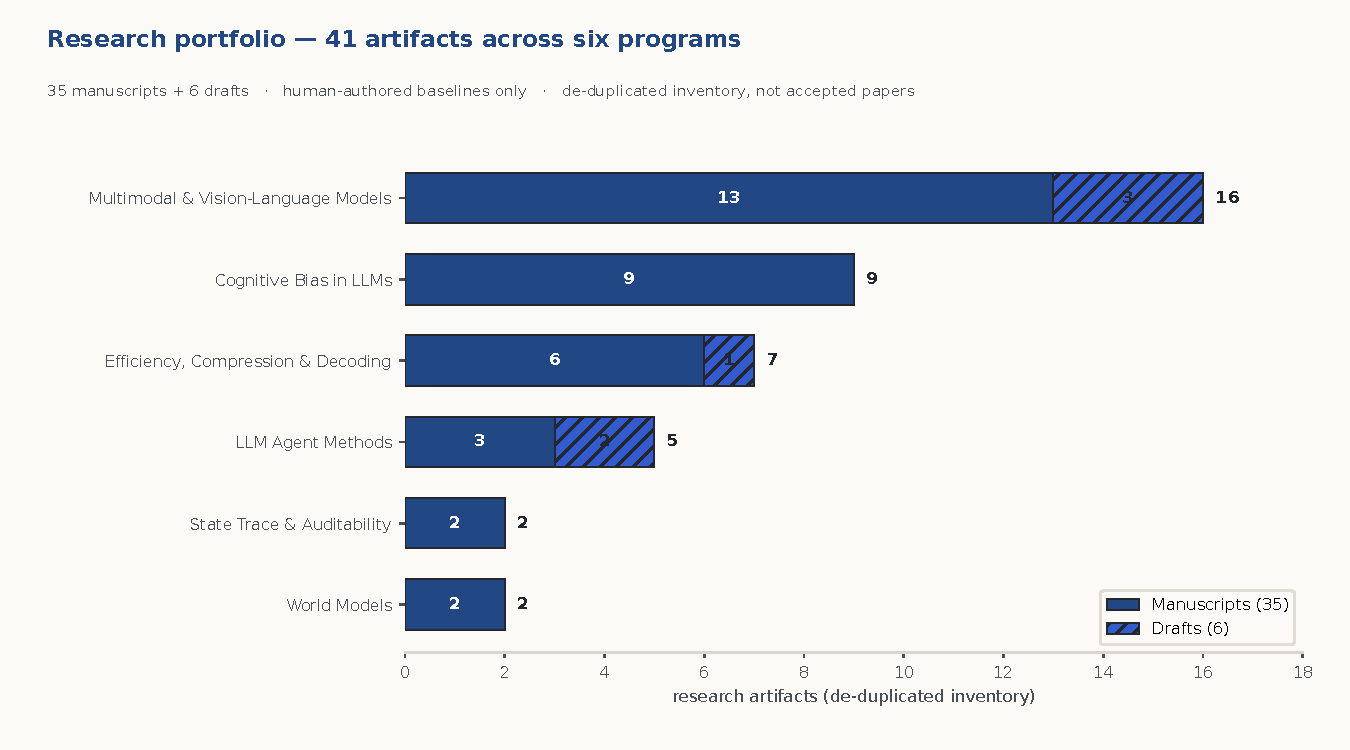
\includegraphics[width=0.70\linewidth]{figures/paper_portfolio.pdf}
  \caption{De-duplicated research-artifact inventory by program and status. The
  chart is generated from \srcpath{evidence/paper\_inventory.json}; manuscript and
  draft labels do not imply external acceptance.}
  \label{fig:portfolio}
\end{figure}

The inventory records sustained output and breadth across task
classes. It does not establish that all artifacts are novel, correct, accepted, or
of equal quality. The count is therefore reported as a production record rather
than a publication metric.
